% Two sided means the left and right margins are different sizes and they alternate every page.
% If your document is printed to be book or spiral bound this allows for a thick spine to not
% eat into the space for your page content.
\documentclass[11pt, a4paper, oneside]{custard}

\usepackage{geometry}
\usepackage[utf8]{inputenc}
\usepackage[T1]{fontenc}
\geometry{
	a4paper,
	left   = 30mm,
	right  = 30mm,
	top    = 30mm,
	bottom = 30mm
}

% All imports, packages, and configuration in here.
% Your document should be about content so we abstract away the styling rules and tools we are using.
%% Here you can specify new commands and environments that you intend
%% to use. Using commands can make your document easier to write, read
%% and be more consistent.

\usepackage[linesnumbered,ruled]{algorithm2e}
\DeclareMathOperator*{\argmin}{arg\,min}

\usepackage{diagbox}
\usepackage{appendix}
\usepackage{textcomp}
\usepackage{setspace}
%\usepackage[document]{ragged2e}
\usepackage{verbatim}
\usepackage{multirow}
\usepackage{multicol}
\usepackage{booktabs}
\usepackage{enumitem}
\sloppy
\usepackage{graphicx}
\usepackage{threeparttable}
\usepackage{epsfig}
\usepackage{epstopdf}
\usepackage{float}
\usepackage{enumitem}
\usepackage{cite}
\usepackage[export]{adjustbox}
\usepackage{algorithmic}
\usepackage[nohyperlinks,printonlyused]{acronym}
\usepackage{amsmath}
\usepackage{amsfonts}
\usepackage{array}
\usepackage{tabularx}
\usepackage{xltabular}
\usepackage{longtable}
\usepackage{times}
\usepackage{amssymb}
\usepackage{hhline}
\usepackage{color}
\usepackage{soul}
\usepackage{colortbl}
\definecolor{Gray}{gray}{0.85}
\usepackage{rotating}
\usepackage{fix2col}
\usepackage{pdflscape}
\usepackage{pdfpages}
\usepackage{stmaryrd}
\usepackage[export]{adjustbox}
\usepackage{bbm}
\usepackage{relsize}
\usepackage{xfrac}
\usepackage{bibentry}

%\usepackage{refcheck}

%watermarking
\usepackage[english]{babel}
\usepackage{tikz}

%% Uncomment the following line for hyper links - not recommended for printing
\usepackage[colorlinks, linkcolor=, anchorcolor=, citecolor=, filecolor=, menucolor=, runcolor=, urlcolor=]{hyperref}

\setcounter{tocdepth}{1}
%\setcounter{minitocdepth}{3}
\linespread{1.31}

\newcommand\litem[1]{\item{\bfseries #1:\enspace}}

\interdisplaylinepenalty=2500

\newcolumntype{L}[1]{>{\raggedright\let\newline\\\arraybackslash\hspace{0pt}}m{#1}}
\newcolumntype{C}[1]{>{\centering\let\newline\\\arraybackslash\hspace{0pt}}m{#1}}
\newcolumntype{R}[1]{>{\raggedleft\let\newline\\\arraybackslash\hspace{0pt}}m{#1}}

\renewcommand{\thefootnote}{\fnsymbol{footnote}}
\setlength{\LTpre}{-10pt}\setlength{\LTpost}{-30pt}%
\newcommand{\oiint}{\begin{picture}(0,0)(-10,-2)\put(0,0){\oval(12,8)}\end{picture}\iint}
\renewcommand{\mathbf }{\boldsymbol}

\def \eg{e.g.\ } % Allows you to write \eg in LaTeX instead of typing e.g. so that every single one will be formatted the same.
\def \Eg{E.g.\ } % Define some other common variants. If you later want to change one of these definitions,
\def \ie{i.e.\ } % it will update all the usages throughout the document.
\def \Dr{Dr.\ }
\def \vs{vs. }
\def \etal{\emph{et al.\ }}
\def \sota{state-of-the-art }
\def \handcrafted{hand-crafted }

\usepackage{listings,lstautogobble}
\usepackage{sourcecodepro}
\pdfmapfile{=SourceCodePro.map}
\lstset{
	xleftmargin=0.5cm,frame=tlbr,framesep=4pt,framerule=0.5pt,
	language=,
	upquote=true,
	columns=fixed,
	tabsize=2,
	extendedchars=true,
	breaklines=true,
	numbers=left,
	numbersep=10pt,
	basicstyle=\ttfamily\scriptsize,
	numberstyle=\tiny,
	stringstyle=\ttfamily,
	captionpos=b,
	showstringspaces=false,
	autogobble=true
}

\usepackage[font=small,skip=10pt]{caption} %,format=hang
%\usepackage[labelformat=simple]{subcaption}
\usepackage[labelformat=simple]{subfig}
%\captionsetup[figure]{format=hang}
%\captionsetup[lstlisting]{format=hang}
\renewcommand{\thesubfigure}{\Alph{subfigure}.}

\renewcommand{\thefootnote}{\arabic{footnote}}

% Use IEEEtran citation style.
\bibliographystyle{IEEEtran}

\def\samplefont#1{%
    % set font style and save name
    #1\edef\savedname{\fontname\font}%
    % print small sample
    {\leavevmode\tt\hbox to 1in{\savedname:\hss}}%
    abcxyz ABCXYZ 123\par
}


\begin{document}

% The custom data for Swansea University and your degree name.
% The \protect\\ command forces a new line in the title which might be otherwise overriden by the template
	\title{Walking Aid Usage Prompt System}
	\author{Pedro Caetano, Matthew Culley, Sean Coaker, Panayiotis Melios}
	\awardinginst{Swansea University}
	% Comment / uncomment your degree type as needed.
	\degree{Masters of Science}

% Institution details and logo
	\department{Faculty of Science and Engineering}
	\university{Swansea University}
	\unilogo{graphics/swansea.png}

% Hard code the date or allow the LaTeX compiler to fill it in whenever you recompile the document.
	\date{\today}

% Build the title and declaration pages, and pad the document so the text starts on a right hand book page.
% Page numbering is in roman numerals until the first page of an actual chapter which resets numbers
% starting from 1 at that point.
	\frontmatter%
	\maketitle
	%\cleardoublepage
	\tableofcontents

% Optionally you can make a bank of known acronyms in acronyms.tex that you can call on throughout your document.
	%\input{acronyms}

% Reset numeric page numbering from page 1
	\mainmatter%

% Insert the code for each of your chapters
	\chapter{Topic} \label{ch:topic}

    This chapter details the problem and task our project aims to solve along with the limitations that could affect
    our project, including an analysis of the current solutions our project has to compete with.\ We will provide
    background research on dementia patients and senior citizens with similar conditions (hereby depicted as the
    'User(s)') and their issues with forgetting their walking aids, and how wearable devices can have a varying
    psychological impact on them.\ Finally, we will detail our current progress consisting of two initial meetings
    with our client, and our takeaways from these engagements.

    \section{Background}

        The client came to us with the idea of developing a product for those suffering with dementia, a syndrome that
        is usually associated with a declining functionality of the brain.\ Dementia can manifest itself with a large
        range of symptoms, most commonly including memory loss, loss of mental sharpness, or loss of the use of
        language~\cite{nhs_choices}.\ More importantly to our project, one other symptom can be a loss in movement
        skills, or an increased difficulty in moving.\ Dementia has been recognised as an illness that causes an
        increase in falls within
        patients~\cite{doorn_gruber-baldini_zimmerman_hebel_port_baumgarten_quinn_taler_may_magaziner_et_al._2003}.\ As
        dementia affects mainly more elderly population, falls are often more dangerous to them.\ It is therefor not
        uncommon for dementia patients to be using walking aides to help mitigate this, a walking aid is only effective
        if it is used by the patient, and as explained by the client, this is something the users may struggle with
        remembering to use

    \section{The Problem}
        Upon completion of our initial meeting with the client, we clarified the motivation behind this project and the
        problem that we are working together to solve.\ The problem is to develop a solution that detects when a
        user is moving without their walking aid and reminds the patient (with a recorded message by a
        friend or a relative) to take their walking aid with them.\ Initial discussions between ourselves and the client
        identified current issues with users feeling uncomfortable in being forced to wear foreign objects,
        meaning we would need to take this into account when developing our solution.\ We also clarified that users get easily alarmed and frightened by generic “obnoxious” alarms, often associating them with those
        notifying them of danger, such as fire alarms.\ The client suggested that we facilitate a recording feature
        within our solution that would allow recognisable voices to the user to remind them to use their
        walking aid.

        \subsection{Similar Solutions}
            Current solutions include the use of locator systems that allow users to easily track down valuables such as
            keys or a wallet.\ Such systems include the Tile ecosystem which allows a user to attach a Tile device to
            their valuables and then use a smartphone app to trigger an alarm from the Tile device that notifies the
            patient of the location of their valuable.\ As previously mentioned, users can get frightened and
            disorientated by the sounds of alarms often associating them with danger rendering these forms of solutions
            unsuitable for our problem.\ This is without considering how difficult a users mind finds navigating through
            a smartphone device to open an application and request their Tile device to ring an alarm to help them
            identify the location of their valuable.\ Another problem with such approaches, is the lack of functionality
            for sending an alarm to the patient if they start walking without the aide.\ Solutions such as Tile would
            help a patient find the aide if it had been misplaced but implementing functionality to remind the patient
            to find the aide if they have already started walking without it, is lacking entirely.\ Other more legacy
            systems that carers may use to notify themselves that their patient is moving include hanging items from
            door frames that clatter together when the patient walks through the door or adding pressure pads under door
            mats that sound an alarm when the patient steps on the door mat.\ Our solution is focussing on the protection
            of users that are alone and wanting to move around their home or ward, meaning that door mat pressure pad
            based solutions and methods for alarming a carer would be insufficient.\ We also would like our design to be
            more elegant than those rudimentary solutions, if the patient is walking with the aide, they will still get
            an alarm from the pressure pad.\ A well implemented system could alleviate both those problems, and increase
            the quality of life of the patient and facilitate the carer.

        \subsection{Limitations}
            Our main limitation for our project is that we need to develop a discrete device that will not make the
            users feel uncomfortable in any way and will minimise discomfort to an extent where it is
            acceptable for day-to-day life.\ Early plans for the device lean towards a watch style device that the
            patients can wear on their wrist to track their movement.\ If we were to create a wrist wearable device
            then we would need to ensure that the footprint of device is small enough to be worn comfortably.\ This limits
            the hardware that we can feasibly use for our project.\ We also need to consider the hardware being
            used and how they can all be fit within a wrist device.\ The head of Swansea University’s Embedded Systems
            module has kindly offered to supply us with ESP32 based TinyPICO devices which would be suitable for this
            project due to their small form factor.\ We would need to consider how an accelerometer could be attached to
            the TinyPICO to allow both devices to fit within a watch casing.\ If we could find hardware small
            enough to build into a watch-based prototype, we may still run into issues with the patients wanting to use
            the product.\ During our meeting we were told that patients already had to wear wrist tags or similar items.
            Adding more items the patient needs to wear is unlikely to be well received.\ Our form factor could take the
            shape of something that clips onto what the patient is already wearing, such as clothes or belts, or a tag
            that they already use.

            Other limitations for the wrist device are that it should not contain any strong LEDs, obnoxious vibration
            motors or alarms to avoid startling the user.\ Avoiding the use of LEDs would be of benefit to us here as it
            would allow the watch device to save battery during operation.\ Another limitation to the watch device is
            that it would need to be power efficient and avoid the users needing to frequently charge the device.\ The
            patient needing to do this would work against our goal of creating a user-friendly experience for them.\ The
            ESP32 chips included on the TinyPICO boards utilise a facility called 'deep sleep' or hibernation states,
            which effectively powers down certain modules connected to the board.\ We could create a system here that
            fires an interrupt when the accelerometer detects movement, then forcing the ESP32 to wake up and handle the
            interrupt.\ The device could therefore be in sleep whilst the patient is static, to save battery.

            The device attached to the walking aid has much less limitations, and so we do not need to consider such a
            small form factor as it is not being worn but will still be using a TinyPICO to encourage compatibility and
            interchangeable/modular development experiences.\ Our limitation with this device is to also disable the use
            of LEDs to avoid startling the patients, and to include a speaker and microphone to allow a relative or
            carer to record a voice note which will be played to remind the patient to take their walking aid with them
            when moving.\ The TinyPICO boards include a very minimal amount of storage space and so we may need to
            include a SD card to store the recordings.\ We will also be limited to the budget of £150 that we have been
            assigned and must ensure that all the devices needed to build the system can be purchased within our budget.

    \section{Current Work}
        As stated earlier in this chapter, we have held initial meetings with the client where we have clarified the
        problem they aim to solve with this project and outlined the project scope.\ On the 18th of November we held an
        introductory meeting with the client where we gained an understanding of what the problem is and what kind of
        system the client was expecting to be produced.\ We clarified that we would need to gain our supply of hardware
        ourselves and that a budget of £150 would be allocated to us to aid with the procurement of the necessary
        hardware devices.\ However, within this initial meeting we failed to identify the final direction the client
        wanted the project to head down and instead came away with the option of either developing a wearable device
        that would detect when the users was moving, or to use a non-wearable device such as a pressure
        blanket that would detect when the patient had got up from where they were static.\ We agreed with the client
        that we would schedule a second meeting for the 25th of November and within that time analyse the advantages
        and disadvantages to each method of developing the solution.\ We then agreed that we would return with a solution
        that we thought would best suit the design brief and that would best suit the development talent available to us
        within our team.

        Within our own intra-team meeting we decided upon building and developing a wearable device solution over a
        non-wearable solution due to the extra features that could be included into a wearable device such as a fall
        detection system, a system recommended to be included by the client.\ We felt that despite a non-wearable device
        being a plausible route to take the project down, that factors such as a users moving off a pressure
        pad without actually standing up and walking would diminish the effectiveness of our solution.

        On the 25th of November we hosted our second meeting with the client and established the team's preferred route
        for the development of this project.\ The client was content with this and agreed that the solution should be
        developed as a wearable device.\ We finalised the £150 budget with the client and agreed that our next steps
        would be to complete our milestone 1 document, including user requirements, and compiling a list of necessary
        hardware to develop the project.\ Our next meeting with the client is scheduled for December 16th where we will
        finalise the user requirements and compile a list of hardware to be purchased with the budget made available to
        us.

    \section{Project Aims}
        For evaluation purposes at the conclusion of this project, we will detail within this section a list of aims
        that should be met along with lower level objectives that define a set of criteria that will allow use to meet
        said aims.\ An evaluation within milestone 3 will look to compare the final product produced against the aims set
        out in this section in an attempt to gauge how successful our project is.\ A list of our aims and their lower
        level objectives can be seen below.

        \begin{itemize}
            \item Develop a solution that reminds the user(s) to take their walking aid with them when attempting to walk.
            \begin{itemize}
                \item We should create a wearable device that includes a tri axial accelerometer to detect when the
                    user(s) have started moving.
                \item A device should be connected to the walking aid that also contains tri axial accelerometer that
                    will be used to detect if the walking aid is moving whilst the wearable device is moving.
                \item The walking aid device should contain a microphone and speaker that allows a carer to record a
                    reminder for the user(s) in attempt to avoid startling the user(s), which could happen when using
                    generic alarms.
            \end{itemize}
            \item Create prototype devices that avoid startling the user(s) and avoids making them uncomfortable.
            \begin{itemize}
                \item The wearable device should be designed and built such that it is inconspicuous in attempt
                    to not draw attention to it from the user(s).
                \item Unless the user(s) is deaf, we should avoid the use of LEDs, vibration motors, and the use
                    of generic alarms.
                \item The wearable device should be developed to be worn on the wrist rather than on a more
                    uncomfortable body part such as the neck.
            \end{itemize}
            \item Produce a solution that the client concludes is satisfactory.
            \begin{itemize}
                \item Produce a document of user requirements and receive confirmation from the
                    client that the requirements are sufficient.
                \item Allow for changes in requirements during project
                    development.\ Our chosen agile methodology will allow for easy integration of changed user
                    requirements here.
                \item Develop the solution such that it is compliant with the user requirements.
                    \end{itemize}
        \end{itemize}
	\chapter{Requirements} \label{ch:Requirements}

In this section, we will detail the project's functional and non-functional requirements, which are broken down into
higher-level user requirements as well as lower-level specifications that will describe the process our team will go
through to ensure the user requirements are met. These written requirements have been demonstrated to the client and they have provided their consent for the project to be based upon them.

\section{Functional Requirements} \label{sec:func_requirements}

\vspace{1em} \small
	\begin{xltabular}[H]{\textwidth}{c | X | X | X}
		\caption[Functional Requirements.]{A table of functional requirements split into user requirements and their relevant specifications needed to meet those user requirements, along with the progression made so far.}\\

		\toprule

		Code & User Requirement & Specification & Progress\\

		\midrule
		\endfirsthead

		\toprule

		Code & User Requirement & Specification & Progress\\

		\midrule
		\endhead

		\hline
		\multicolumn{4}{|r|}{{Continued on next page}}\\
		\hline
		\endfoot

		\bottomrule
		\endlastfoot

        FREQ1

        &

        The wearable device should detect when a patient has walked more than 1 metre before communicating with the walking aid.

        &

        We can use a tri axial accelerometer to detect changes in acceleration that are indicative of the user moving or being mobile. Once movement is confirmed, we will then commuicate with the walking aid device to ensure the user has successively reached and engaged with it, prior to alerting them to use it.

        &

        -\\

        \midrule

        FREQ2

        &

        Patients should be alerted with the voice of a friend, carer or relative to avoid startling them.

        &

        The device to be attached to the walking aid should include a microphone and speaker that will allow the user to record a voice note and store it on the device. We may need to include an SD card within this device that will store the voice note if need be.

        &

        -\\

        \midrule

        FREQ3

        &

        The wearable device should include a solution for deaf people that still reminds them to take their walking aid with them without the need for an audio alarm.

        &

        The wearable device could use a vibration motor here that vibrates to remind the user to use their walking aid. We can also utilise the LEDs on board the TinyPICOs to flash to remind the user also. There are issues here with potentially startling the patient with the use of vibration and LEDs, however we feel this is most feasible method for meeting this user requirement.

        &

        -\\

        \midrule

        FREQ4

        &

        If development time allows, the system should include fall detection as a stretch goal feature.

        &

        Using the tri axial accelerometer mentioned in the specification of FREQ1, we could detect acceleration and movement along the negative side of the y-axis in attempt to detect when the patient has fallen. An alert system can be used in accordance to alert a nearby carer or relative.

        &

        -\\

        \midrule

        FREQ5

        &

        The wearable device should communicate to the walking aid device to let it know when it's started moving.

        &

        To meet this requirement we investigate the use of 433MHz Rx/Tx modules for low power and low level communication between the 2 devices in the system, this technology should allow for the basic level of communication required, with minimal power use and minimal complexity.

        &

        -\\

	\end{xltabular}
	\label{tbl:func_reqs_table}
 \vspace{5em}

\section{Non-Functional Requirements} \label{sec:non_func_requirements}

\vspace{1em} \small
	\begin{xltabular}[H]{\textwidth}{c | X | X | X}
		\caption[Non-Functional Requirements.]{A table of non-functional requirements split into user requirements and their relevant specifications needed to meet those user requirements.}\\

		\toprule

		Code & User Requirement & Specification & Progress\\

		\midrule
		\endfirsthead

		\toprule

		Code & User Requirement & Specification & Progress\\

		\midrule
		\endhead

		\hline
		\multicolumn{4}{|r|}{{Continued on next page}}\\
		\hline
		\endfoot

		\bottomrule
		\endlastfoot

        NONFREQ1

        &

        The watch should be a small enough form factor to fit on the wrist of the patient.

        &

        Deciding to use TinyPICO devices as the main board of the device will allow us to keep the device to a small form factor given the TinyPICO is 18mm x 32mm. We will also take into account the form factor when deciding upon extra hardware to add to the devices.

        &

        -\\

        \midrule

        NONFREQ2

        &

        The devices shall be power efficient to avoid the patient needing to charge them often.

        &

        The TinyPICO devices we will use as the main boards for the devices include an ESP32 chip capable of using deep sleep cycles. These cycles allow the ESP32 to power down non critical components in order to save power. We can create an interrupt within the code here that powers the devices on when an alarm needs to be fired due to the patient moving. This means that the devices will only need to be fully powered on when movement is detected.

        &

        -\\

        \midrule

        NONFREQ3

        &

        The devices shall avoid startling the patients with the use of LEDs and vibrations unless they are deaf.

        &

        In this case we would power down the LEDs and Vibration motor at all times to avoid startling the patient. Powering down these devices will also allow us to save battery.

        &

        -\\

        \midrule

        NONFREQ4

        &

        The wearable device should be discrete enough that it does not make patients uncomfortable wearing it.

        &

        We intend to design the device to make it as close the design of a watch as possible, keeping it small and sleek so that it looks like a fashion accessory rather than a medical device. Using small hardware devices we can keep a small form factor so that the device is not overly noticeable on the patient's wrist.

        &

        -\\

        \midrule

        NONFREQ5

        &

        Security of devices should prohibit outside devices from communicating with the network.

        &

        A possibility here is using an agreed upon 'sync word' between our 2 devices that only reads communcations from devices using the same 'sync word'. This would stop other devices being able to communicate with the network unless they knew the sync word being used.

        &

        -\\

		\midrule

        NONFREQ6

        &

        The developed prototype wearable device shall be designed such that it can fit various wrist dimensions.

        &

        The strap of the wearable device should be designed such that it can be adjusted in a similar way to how normal watches can be adjusted.

        &

        -\\

		\midrule

        NONFREQ7

        &

        The coding system the devices run on should be efficient enough to react to real time actions.

        &

        Our code should be developed with efficiency in mind that will allow for real time readings from the accelerometer to precisely detect when movement has passed 1 metre in order to notify the walking aid device that this has happened. The Rx/Tx communication module will allow for fast communication between the devices to ensure that user is promptly reminded to take their walking aid with them.

        &

        -\\

		\midrule

        NONFREQ8

        &

        The system should be delivered upon its conclusion with relevant documentation, including a user manual.

        &

        Our milestone 3 document will include the necessary documentation needed to be handed over to the client upon the handover of our project. This milestone will include a user manual along with any designs and testing documentation that were created during the development of the product.

        &

        -\\

	\end{xltabular}
	\label{tbl:non_func_reqs_table}
 \vspace{5em}

	\chapter{Specification}\label{ch:specification}
    \section{Description}

        This project includes the development of a wearable device that is able to detect when the user is/has moved,
        and a remote device attached to their walking aid, that is able to remind them to use it if they have not done
        so.\ A prerecorded message from a family member or relative will act as the notification.\ Both devices have to
        be discrete and unobtrusive, as the users are known to be easily startled by new and foreign devices near them,
        as well as with lights/vibration and other stimulus easily confusing them.\ The message will be stored locally,
        either on the hardware products inbuilt storage, or an external SD card.\ In the eventuality that the user is
        deaf or hard of hearing, the device will also have to have support for alternatives stimuli, such as vibration
        or light based feedback.\ Within this section we will provide a brief specification of the project along with
        references to requirements specified in chapter~\ref{ch:requirements}.

    \section{Software Behaviour}
        The wearable device must be able to communicate with the walking aid device for the project to be successful
        (FREQ5). \This communication should occur once the wearable device has detected that the user has walked more
        than 1 metre (FREQ1).\ Then, the wearable device should communicate with the walking aid device to check if the
        walking aid is moving also.\ If it's not, then the walking aid device will play a pre-recorded message from a
        carer, friend or relative reminding the user to take their walking aid with them (FREQ2).\ Once the walking aid
        begins movement then the reminder will stop being played.

        Furthermore, dementia effects all types of people at varying ages.\ That means that the wearable device must be
        able to fit on anyone's wrist and must contain hardware small enough to allow the wearable to fit comfortably on
        the wrist (NONFREQ1).\ Because we do not want patients to feel uncomfortable while using the wearable device, it
        will be designed to look like a watch.\ Apart from the device's appearance and dimensions, the device should be
        power efficient, as the patients may forget to charge it (NONFREQ2).\ Aside from the device's appearance and
        dimensions, the wearable device's material must be durable in  case it is dropped.\ That is why the material of
        the wearable device will be ABS plastic, which is an opaque thermoplastic and amorphous polymer and easily printed
        with our printer.

        Should time allow, the device will also include fall detection functionality as part of an agreed stretch goal
        (FREQ4).\ A tri-axial accelerometer will be used to determine the user's hand height, and more particularly the
        device's height.\ If the user's hand is extremely close to the ground, it is likely that the user has fallen, and
        if the device detects that the user has been on the ground for an extended amount of time it will begin an
        emergency procedure to notify an in case of emergency contact.

        In terms of the security of the system, the wearable device and the walking aid device will communicate only
        with each other in pairs.\ This can be achieved by using a unique synchronization mechanism between each device.
        As a result, an external device will be unable to communicate with the walking aid or even the wearable device
        within the network (NONFREQ5).

    \section{Performance}

        Our main concern with the performance of the device is to ensure that the battery usage is kept at a minimum
        level (NONFREQ2).\ We have previously discussed how deep sleep cycles will be used to do this and is necessary to
        avoid issues where the user may forget to charge the device rendering the device useless.\ Other performance
        concerns centre around the communication between our 2 devices, where the process should use a low amount of
        power and should allow for consistent and robust communication (FREQ5).\ Rx/Tx modules will provide the basis to
        meet this performance criteria.\ Finally, the execution of processes by our device should be instantaneous to
        allow the device to detect and respond to real time movements as quickly as possible\. Using a stripped back
        language such as Arduino C or Micropython will allow for this and will allow the developers the inclusion of unnecessary
        overheads within the code that is uploaded to our TinyPICO devices.

	\chapter{Methodology} \label{ch:methodology}
    \section{Software Developement Methodologies}
        \subsection{Development Methodology}
            Due to the nature of our team and project. We thought it best to implement an agile based development
            methodology. As a small team, it is easy for us to communicate with each other about the project, and easier
            for us to be aware of what the other members of our team are doing, key factors for choosing an agile
            methodology. The question then is, which agile based methodology to use? There are a variety of
            methodologies our there each with their own pros and cons, which we will address some of which shortly. But
            based on these we decided to use a scrum-based development methodology. Scrum is a combination of iterative
            and incremental development. Allowing for a best of both worlds approach of having early builds working, but
            also being agile and able to add requirements during the development process~\cite{srivastava_2017_scrum}.
            The scrum methodology is rather simple. To effectively work, it requires collaboration between an appointed
            ‘Scum Master’ and the rest of the team, as well as a ‘Product Owner’. These members will work in close
            collaboration other multiple, continuous iterations of the software build to create a finished product. The
            role of the scrum master is to eliminate impediments~\cite{srivastava_2017_scrum}or in other terms, to
            create the conditions that allow the development team to work in their most effective manner, they take a
            leading role in choosing what sprints the team work on. A typical scrum workflow consists of iterative scrum
            cycles, typically lasting one to three weeks each. Initially a requirements backlog is created.  This is
            done in collaboration with the client and is the documentation that describes all the requirements that the
            software must meet. It is essentially a description of the product that the team are aiming to build. Once
            an initial backlog is created, the scrum cycles can start. As before mentioned, each scrum cycle lasts
            typically up to three weeks. The cycle kicks of with the team, headed by the scrum master deciding which
            requirements to prioritise and implement in the upcoming cycle. The aim is to have a potentially shippable
            product at the end of each sprint, although this may not be possible immediately. Once the team have
            allocated the suitable requirements to the sprint, the sprint begins, the team works on the product, meeting
            each day in what are known as ‘scrums’ to review progress made on each day. At the end of the sprint, the
            team should have made a shippable product. The team will also meet and hold a sprint review, along with the
            product owner. That demonstrates the product and how it has been developed since the last sprint. The team
            will also review the previous sprint, to see if any changes need to be made in anticipation of the next
            one~\cite{nuevo_2011_scrumbased}. In our case, we will be slightly modifying the implementation of scrum.
            The above-mentioned workflow is designed as a framework for full time software developers, which we are not.
            As much as we may perhaps wish too, we will not be able to meet daily to discuss the project. As students it
            is an unrealistic expectation that we will be able to hold daily scrums, but we can still follow the
            methodology. We will aim to hold scrums at frequent intervals, in periods perhaps of every week, to keep
            tabs on the current sprints running. We can also compensate for this by being realistic in what we can
            achieve, and what we set as the sprint’s goals. Ultimately, we chose to use scrum for a variety of reasons.
            Primarily of all, we realised that as a small team, frequent communication would be easy to achieve, so we
            would be able to make use of this framework in the most effective manner, compared to other methodologies.
            We would be able to meet frequently and use that to ensure progress is made on the project. Scrum works well
            with this. Using scrum would enable us to work together to frequently get working products out and allow us
            to put ourselves in a position to implement more features. We also feel that using scrum would allow us to
            have a higher quality product, as the frequent iterations during sprints would allow us to streamline our
            implementation and constantly improve it. It also allows us to minimise risk. Take the waterfall methodology
            for example, where implementation begins a lot later in the lifecycle. Using scrum, where we start
            programming earlier, gives us more time to deal with any difficulties we encounter. It allows us to spot
            problems earlier, have longer to address them, or to have time to plan alternative implementations that
            avoid such problems. We chose scrum over other agile methodologies for a few reasons. But mainly because we
            thought it was the best fit for our team and situation. Other methodologies, like extreme programming, could
            have worked well for us, but didn’t suit our situation as students as well. For example, extreme programming
            requires pair programming, something that would be hard for us to do and would drastically tank our
            productivity. Overall, we made our decision based on what would work best for us as a team.

    
        \subsection{Hardware and Software}
            With regards to hardware and software that we intend to use, we made our decisions based on the experience with
            hardware from previous work. For hardware, our product is going to be made using tiny PICO hardware. Multiple
            members of our group took the Embedded Systems module previously, so we have experience using this hardware. The
            tiny PICO on its own, does not have all the features we need, so we will be using extra hardware to supplement it.
            We will be using accelerometers to measure changes in movement of the dementia patients. We will also be
            implementing speakers and microphones to allow voice recordings to be created and played back. In the same vein, we
            will be using SD storage for storing sound files that can be played back. We also have access to a 3d printer, we
            will use this to create prototype casings for our product. It will enable us to rapidly design and test prototype
            products. This is important, as mentioned before in this document, the form factor of our product is important to
            minimise patient discomfort or resistiveness. Using 3d printing we can quickly test form factors and send prototype
            designs to our client quickly if they have a 3d printer too. This rapid prototyping will be beneficial, getting the
            right form factor is vitally important to ensure that the product is likely to be accepted by dementia patients It
            will help us meet requirement NONFREQ1. We will be using a variety of software too. As is sensible with any product,
            we will be using git for version control and collaboration. Using git has a variety of benefits, version control,
            and enabling proper collaboration in the easiest way. It enables us to work on the same project without having to
            share resources. As mentioned, we are using TinyPICO devices as our hardware. Programming these devices is done in
            the Arduino C language, we will be using the Arduino IDE to program our product. Our document is created with latex,
            shared on git to enable us to collaborate and work on the document together. With relation to our requirements, the
            hardware we use was chosen too directly meet the non-functional requirements that we defined. Tiny PICOs are
            incredibly small and can be fitted in very small form factors such as a watch which is in line with NONFREQ1.
            Accelerometers can also be made in small form factors too, which enables them to also fit in a small casing and help
            us meet our requirements. Tiny Picos are also power efficient, for example, they have various sleep modes that we
            can utilise to minimise power output, by avoiding using items such as LEDs, we can extend battery life, but also
            meet our requirement on not having obnoxious or startling lights or effects, these features help meet NONFREQ2 and
            3. We chose some of the other hardware to meet the functional requirements of the project. Accelerometers can detect
            if the user is walking, helping to meet FREQ 1. And the speaker we will use can play back messages to the user,
            meeting FREQ2. Storage and microphones also enable this requirement to be met.


    

	\chapter{Project schedule}\label{ch:schedule}
    \section{Gantt Chart}
    We built a Gantt Chart for the project schedule to allow us to keep track of the time. We couldn't create tasks that
    would indicate a slippage since it would disrupt the critical path. As a result, we increased the time alloted to
    each assignment, reflecting the slippage. We included slippage due of other university homework, exams and even
    illness.

    As shown in Figure \ref{fig:gantt_chart}, the highlighted tasks illustrate the project's critical path. We devided
    the project into three Sprints because we are utilizing the scrum methodlogy. The first Sprint consists only of
    require collection and project planning. The second Sprint includes the sprint plan, as well as the software and
    hadrware designs and implementations. The third Sprint contains the sprint plan as well as the system's final
    implementation, in which the walking aid will connect with our system, the wrist device. The final task of each
    Sprint is a milestone, signaling the Sprint's completion.

    \begin{figure}[H]
      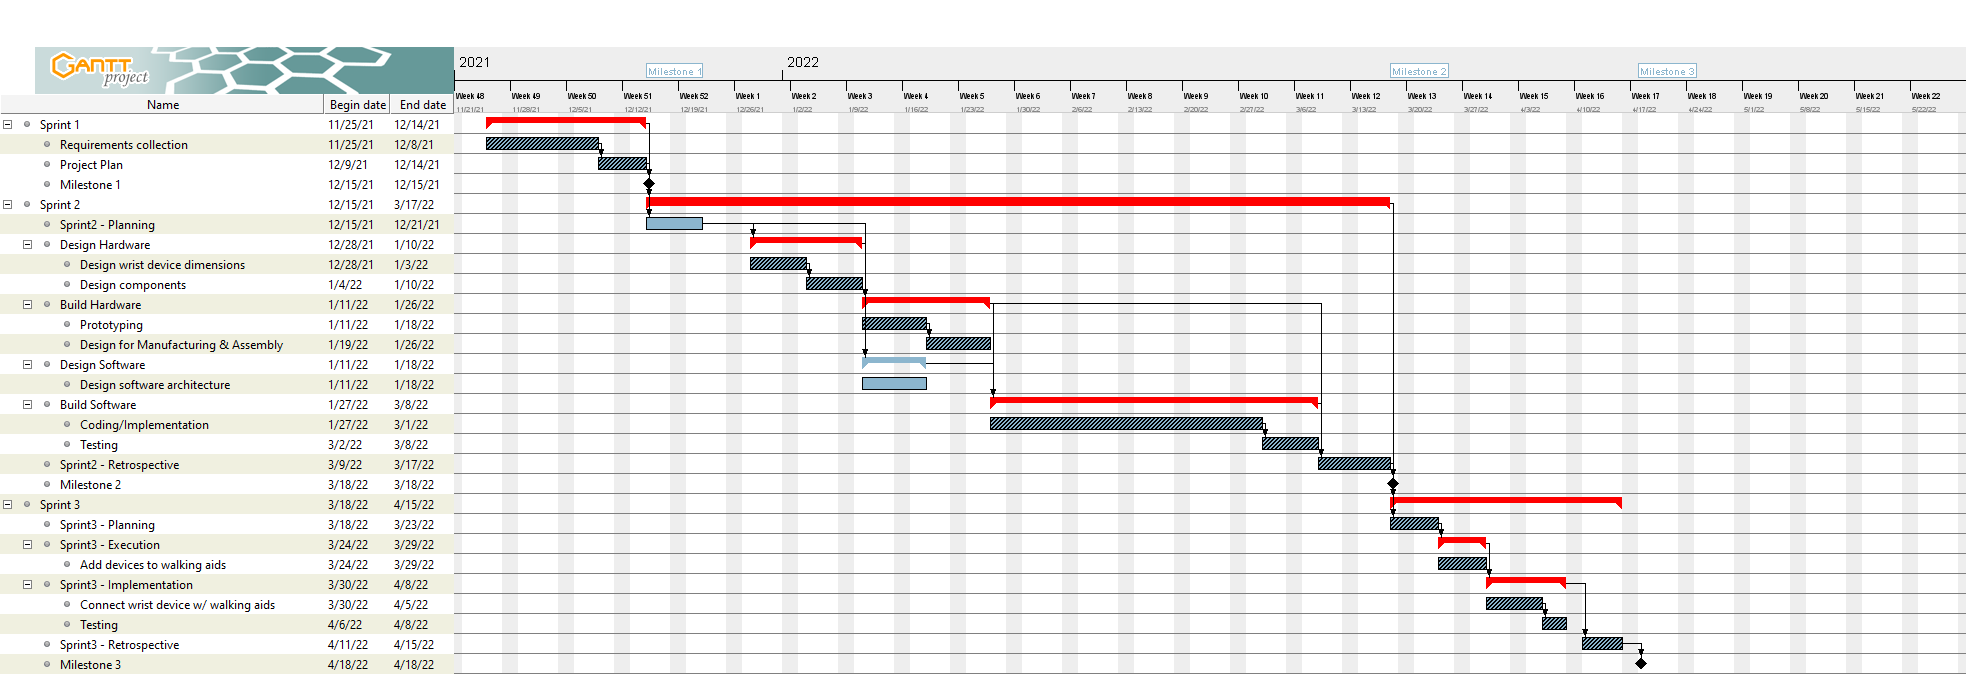
\includegraphics[width=\linewidth]{graphics/Gantt_Chart.png}
      \caption{Gantt Chart}
      \label{fig:gantt_chart}
    \end{figure}

    \section{Activity Network Diagram}

    In terms of scheduling, an activity diagram is just a significant as designing a Gantt Chart. We merged several of
    the jobs that were introduced to Gantt Chart into one task to make the activity network diagram more undestandable.
    However, this has no bearing on the total time requried to finish the project. According to Figure
    \ref{fig:activity_network_diagram}, the total time requried is 107 working days.

    \begin{figure}[H]
      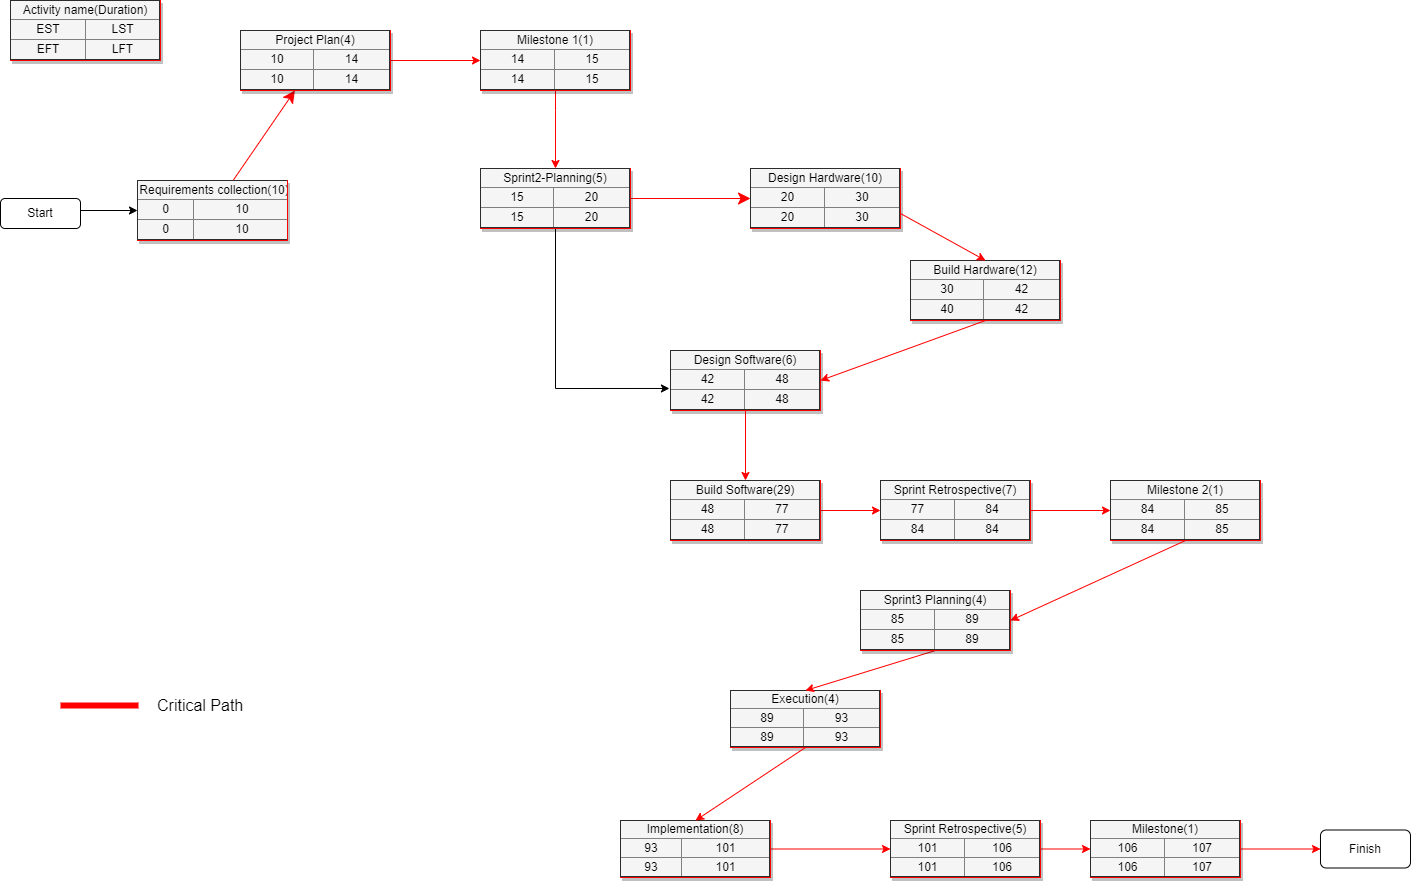
\includegraphics[width=\linewidth]{graphics/AND.drawio.png}
      \caption{Activity Network Diagram}
      \label{fig:activity_network_diagram}
    \end{figure}

	\chapter{Risk Analysis} \label{sec:risk}

In this section, we have completed a review and analysis of the risks from our Milestone 1 document \cite{coaker}. Where necessary, we will detail where we have run into risks, and if so, what steps we took to manage them. We will also detail how progress in the project has affected our risks and how the risks may change moving forwards.

\section{Reflection of Risk since Milestone 1}
Of the risks detailed in Milestone 1 \cite{coaker}, none of them came to pass in a way that affected our project. We did however encounter certain situations that in hindsight should have been included within the original set of risks that we outlined in Milestone 1. These risks will be detailed shortly, but they both share the same general theme; issues with the procurement of hardware for the project. 

The first stumbling block we ran into was with the total price of the hardware we were acquiring being greater than the budget we had been allocated for the project. This should have been a relatively simple risk within the risk assessment that unfortunately we had overlooked. Luckily, we were able to use alternative methods to procure the hardware meaning that the lack of budget did not have a significant effect on the choice or quality of hardware we are using. As mentioned previously in this document, we ended up borrowing two TinyPICOs from the university and using our own funds to purchase the remaining hardware that we need. 

In a similar vein, we encountered another issue with the procurement of our hardware. This time with regards to the time taken for delivery. This was also a slight oversight with regards to our initial time plan as well. The cause of this issue was directly related to the previous issue mentioned, budgetary constraints. With the hardware within the budget being procured via the university, we ran into delays that we had not expected and planned around. As previously mentioned in this document, the hardware took four weeks to arrive, due to being ordered through the university's system, the immediate effect of that being the loss of development time. 

In terms of risk assessment though, these issues do does have a knock on effect on the project going forwards. Multiple of our proposed risks detailed within Milestone 1\cite{coaker} (RSK1, RSK3, RSK8) detail the potential for damage to, or the need to replace hardware. Parts of the mitigation strategies in place for these risks involves having spare room in the budget to replace any faulty or broken hardware as required. As a consequence of the events mentioned prior, we no longer have the space within the budget that allows us to freely replace hardware if required without potentially significant personal financial expense. Compounding this, if we do need to procure additional hardware we may have to deal with the potential for another significant delay. As the university has already made arrangements for the purchasing of the hardware once, we can presume that the delay will not be the same four weeks we initially faced. However, we cannot be sure of this, meaning there is potential for an unknown delay that would be difficult to plan around. This becomes more of a risk as time progresses and our final deadline draws closer. If a crucial piece of hardware were to break with less than a month before the final deadline, it would be extraordinarily difficult to manage.

\section{Amendments to our Risk Assessment}
With this in mind and forethought to what we might encounter further on within the project, we have chosen to revise our risk assessment to ensure we are fully aware of, and prepared to deal with, any risks in the project moving forwards. 

\paragraph{New and Amended Risk}
With the issues previously mentioned in mind, we have decided to extend the risk table to include them. It is important now that we are prepared in the case of hardware failure. In the event of failure the part will need replacing, presumably at short notice. Therefore it is imperative that we have are aware of the correct process of obtaining replacement hardware and agree on how it shall be funded if our budget can no longer cover it. We will also endeavour to avoid making committing changes, (e.g. soldering) until we are one hundred percent confident in what we are doing and have tested the components together first via other means (e.g. on a breadboard). Integrating these management solutions into our workflow will minimise the risk of accidentally "bricking" the hardware we are using.

Since the delay in ordering components resulting in us losing development time for the project, there is now a risk of insufficient time available for the adequate completion of the project. This is relatively straightforward to manage however; frequent and effective communication, as well as regular organised meetings to discuss and manage progress on the project should ensure that we are familiar with the status of the project and whether or not we are falling behind schedule. 

Some of our risks identified in Milestone 1 need adjustment in the mitigation strategies as time remaining on the project diminishes. The mitigation strategies obviously vary depending on the risk, but the general theme is to ensure we are aware of the immediate actions to limit the damage of the risk and rectify it in as little time as possible. For example, in the event of a replacing hardware, we should already be aware of the correct channels to purchase replacements from as well as how the replacements are to be funded. This is important to know before the risk occurs, so that our response can be instantaneous. For the sake of succinctness, we will not detail all such changes in their entirety here, but will highlight the changes in the next section in the document. 

\section{Revised Risk Assessment}

\paragraph{Risks}
Based on our reflections and new amendments to our perceptions of risk within the project, we have made changes to our risks and risk management strategies. We have included the risk table, highlighting any amendments from Milestone 1 \cite{coaker} in bold script.

\vspace{3em} \small
\begin{xltabular}[H]{\textwidth}{c | X | X}
    \caption[Risks Table]{A table of risks along with strategies to mitigate those risks.}\\

    \toprule

    Code & Risk & Mitigation\\

    \midrule
    \endfirsthead

    \toprule

    Code & Risk & Mitigation\\

    \midrule
    \endhead

    \hline
    \multicolumn{3}{|r|}{{Continued on next page}}\\
    \hline
    \endfoot

    \bottomrule
    \endlastfoot

    RSK1

    &

    Our hardware devices may fail and will limit development and testing.

    &

    To mitigate this risk we will choose to use low cost but still effective hardware, which will allow for extra funds within our £150 budget should we need it to replace hardware during development. We also have the opportunity to attain TinyPICO devices from the University for this project, allowing us to minimise the effects on our budget. \textbf{The processes for ordering and funding replacement hardware should be known in advance of the event of any piece of hardware being broken. }\\

    \midrule

    RSK2

    &

    The Rx/Tx modules could fail disabling communication between the wearable and walking aid devices.

    &

    The replacement of these modules should not be much of an issue due to their low cost. The real issue would arise when an Rx/Tx module fails whilst in operation for a patient. We would need to form a protocol here that detects when communication is unable to occur between the 2 devices, and can alert the patient's carer of this.\\

    \midrule

    RSK3

    &

    Uploading erroneous code to our TinyPICO devices could brick the TinyPICO devices.

    &

    Should this occur, we could attempt to reflash previosuly working code onto the TinyPICO. If this fails, we would be left with the occurrence of risk RSK1 where we would need to replace the TinyPICO devices that have been bricked. The low cost of the TinyPICO devices should enable us to purchase some replacements if need be.\\

    \midrule

    RSK4

    &

    GitHub experience a malicious attack or a server failure which could cause our repository to be lost.

    &

    Mitigating this risk is difficult. It's unlikely this will happen and that we would lose our repository as GitHub likely uses a vast backup storage solution. But, should it happen it would be catastrophic and so we should mitigate against this risk. To do this, each developer within the team will store a clone of the repository on their personal system and the team will be able to piece the code back together should this risk arise.\\

    \midrule

    RSK5

    &

    The user requirements we accept could be too large to implement within the given time frame for the project, potentially leaving the client disappointed at project handover.

    &

    To mitigate against this risk, we have discussed our user requirements with the clients and feel that we have decided upon a set of features that we feel we can confidently implement within the time frame given to us. We have also some marked some features as stretch goals to ensure that the most important features are added first. \textbf{There will be frequent communication between group members to ensure everyone is aware of progress and any delays that might affect feature implementation.}\\

    \midrule

    RSK6

    &

    University commitments could impact the development and testing of the product.

    &

    We have attempted to account for this within our schedule by allowing for slippage. Slippage time could allow for the development of unfinished features. We could also spread unfinished work between developers as extra work in an attempt to complete the development of features on time. \textbf{Testing should be planned in advance when group members have time, so that when the testing needs to be carried out, it can be done quickly and efficiently. We are planning to run integration testing now throughout the remaining development of the project.}\\

    \midrule

    RSK7

    &

    The hardware we choose to use may lack the libraries and compatibility with other hardware for quality feature development.

    &

    To avoid this, we will select hardware that is compatible with the Arduino ecosystem to ensure that they are compatible with each other and that libraries are available for code development.\\

    \midrule

    RSK8

    &

    Natural disasters could bring about the loss of hardware and software being used for the development of our product.

    &

    The use of low cost hardware in this system will allow us to replace any compromised hardware if need be. We have decided to store the team's code in a GitHub repository which will allow our code to be protected in an off cite facility. The loss of developer computer systems is by far the biggest risk here, as our budget would not be able to cover the replacement of such computer systems.\\

    \midrule

    RSK9

    &

    Especially in the current coronavirus climate, our developers may be unwell for a period of time that has a negative impact on the development of the project.

    &

    Within our schedule we have included time for slippage that should allow for any time needed by the team to be taken off due to illness. Should a developer need to self isolate and should they not be experiencing symptoms, they could continue to work on the product from a remote location using the GitHub repository.\\

    \midrule

    RSK10

    &

    An Inadequate testing strategy could allow unidentified bugs to be released in the product when handing it over to the client. This could lead to a disappointed client.

    &

    To mitigate against this risk we have devised a testing strategy that ensures thorough testing is carried out throughout the development of our product. We are confident that the proposed testing strategy will allow the team to identify and correct errors in the system before the product is released to the client. \\

    \midrule

    RSK11

    &

    Poorly developed code could mean that despite substantial testing, many bugs could still be included in the product at the conclusion of the project lifecycle, leaving our product to be ineffective for the uses that the client requires.

    &

    To mitigate this risk, we will be following our testing strategy outlined in this document to allow for integration testing. This means that testing will take place every time a new feature is added to the system, allowing us to detect bugs quickly as features are implemented. \textbf{Code should be reviewed by another group member to aid in spotting any major bugs or errors.}\\

    \midrule

    RSK12

    &

    The wearable device we create may cause patients to feel uncomfortable limiting their use of the device.

    &

    We are slightly out of control with this risk as it mainly depends on how the patient reacts to the wearable. Having said this, we aim to make the wearable as discrete and as watch like as possible in an attempt to avoid the patient feeling uncomfortable when wearing it.\\

    \midrule

    RSK13

    &

    Our device could startle or scare the patient putting them in danger.

    &

    We have taken on board the advice of the client for this risk and will be ensuring the watch does not use vibrations or LEDs unless the patient is deaf. We will ensure that generic alarms are not used also in an attempt to avoid startling the patient.\\

    \midrule

    RSK14

    &

    One of our developers could leave the institution, lowering the number of developers we have available to work on the project.

    &

    Should this occur, we would definitely need to use the slippage time we have allowed for in our schedule. We would not be able to bring another developer into the team and would therefore need to share the workload of the developer that is leaving to the other developers on the team. \textbf{We will ensure that all of the group are familiar with what each other is doing, so that in the need to take over from a member on short notice, the transition will be quick, and seamless.}\\
    
    \midrule

    \textbf{RSK15}

    &

    \textbf{Delays in ordering replacement hardware could cause the project to fall irreparably behind schedule.}

    &

   \textbf{Steps to mitigate RSK1 and RSK3 should be followed. To minimise chances of "bricking" hardware, permanent, difficult to undo processes should only be completed when necessary and the system relying on those parts has been properly tested to ensure no damage will occur. We have also already acquired multiple sets of devices to ensure that we have fallback hardware if necessary.} \\
   
    \midrule

    \textbf{RSK16}

    &

    \textbf{Due to previous delays, insufficient time to adequately complete the project.}

    &

   \textbf{Frequent communications and meetings should be held to ensure the group are familiar with the current status of the project, with weekly meetings already being booked, and how well the project is following the agreed upon time plan. In the event of falling behind irreparably, communication with the client is important to ensure that the product produced is as useful as possible.}\\

\end{xltabular}
\label{tbl:risk_table}
 \vspace{6em}

\paragraph{Risk Matrix}
As a whole, it is important to realise now that with time on the project diminishing, the impacts of risks we may encounter is only going to increase. We will have less time to manage or action the mitigation plan. Luckily within our time plan we allocated a certain amount of slippage time that we can use to deal with any risks we would encounter. Unfortunately, we have already been forced to use some of this time as a result in the delay in procuring hardware. We are confident that we have managed to recoup some of that time, but there is no doubt that we do not have as much now as when we started. Within the updated risk matrix below, an increase in impact is marked in italic. New risks have been marked in bold.


\vspace{3em} \small
\begin{xltabular}[H]{\textwidth}{X | X | X | X}
    \caption[Risk likelihood/impact matrix]{A matrix detailing the likelihood of a risk occurring along with the relative impact caused by that risk occurring.}\\

    \toprule

    \diagbox[innerwidth=3.2cm]{Likelihood}{Impact} & Low & Medium & High\\

    \midrule
    \endfirsthead

    \toprule

    \diagbox[innerwidth=3.2cm]{Likelihood}{Impact} & Low & Medium & High\\

    \midrule
    \endhead

    \hline
    \multicolumn{4}{|r|}{{Continued on next page}}\\
    \hline
    \endfoot

    \bottomrule
    \endlastfoot

    Low

    &



    &

    RSK4, RSK7

    &

    \textit{RSK2}, RSK8, RSK13, RSK14\\

    \midrule

    Medium

    &

    RSK12

    &

 

    &

    RSK1, \textit{RSK3}, RSK5, RSK10, RSK11, \textbf{RSK15}, \textbf{RSK16}\\

    \midrule

    High

    &



    &

    RSK9

    &

    RSK6\\

\end{xltabular}
\label{tbl:risk_matrix}




% Formatting citations properly when they are rendering incorrectly in your PDF can be fiddly,
% espectially when punctuation and international characters are involed. Sometimes multiple re-compilations
% are needed in addition to clearing temporary auxiliary files to see your changes in your document.
% Insert the bibliography using citations contained in the file citations.bib
	\bibintoc
	\bibliography{citations}

\end{document}
